\subsection{Các khó khăn so với bài toán truy xuất hình ảnh cơ bản}

Mặc dù bài toán truy xuất địa danh thường được đánh giá và phát triển dưới góc nhìn là một bài toán truy xuất hình ảnh hoặc truy xuất thực thể, để biến đổi các giải pháp cho bài toán truy xuất hình ảnh thành giải pháp cho bài toán này, chúng ta cần phải đề xuất các hướng phát triển để triệt tiêu các khó khăn gắn liền với bản chất của dữ liệu địa danh. Khi nhận diện dữ liệu địa danh trong tập dữ liệu huấn luyện thành thị, mô hình học sâu sẽ phải xử lý một lượng lớn dữ liệu chứa các yếu tố lặp đi lặp lại đến từ kiến trúc nhân tạo như đường phố và cơ sở hạ tầng. Khi xử lý dữ liệu được thu thập trong một khoảng thời gian dài, mô hình học sâu cần đảm bảo tính bền vững của các đặc trưng biểu diễn trước các yếu tố thay đổi về điều kiện môi trường và phong cảnh được tạo ra do nhiều yếu tố phức tạp như mùa màng, thời tiết, thời gian, ánh sáng, \dots Ngoài ra, dữ liệu đại diện cho các đối tượng địa danh mà mô hình cần học thường được thu thập từ các góc nhìn khác nhau với thiết bị và cảm biến khác nhau, yêu cầu khả năng khái quát hóa cao của mô hình học sâu. Quá trình phát triển để tăng cường độ bền của đặc trưng biểu diễn trước các thay đổi trong điều kiện tự nhiên, môi trường, xã hội, thiết bị thu thập dữ liệu, \dots đã đặt bài toán truy xuất địa danh vào một phân loại khác biệt so với bài toán truy xuất hình ảnh cơ bản. Trong phần này, chúng tôi sẽ trình bày các khó khăn đặc trưng của bài toán truy xuất địa danh và các hướng phát triển để giải quyết các khó khăn này, lấy cảm hứng từ các giải pháp đã được đề xuất cho bài toán truy xuất hình ảnh cơ bản và các bài toán khác.

\subsubsection{Chọn vật thể và góc nhìn}

Tập dữ liệu hình ảnh địa danh cần xử lý trong bài toán truy xuất địa danh mang nhiều yếu tố lộn xộn (clutter), gây nhiễu, tạo ra hiện tượng phân tâm trực quan (visual distractors) cho các mô hình. Từ những ngày đầu phát triển, các nhà nghiên cứu đã ghi nhận mức độ quan trọng của quá trình quan sát và chọn ra các thành phần, góc nhìn của ảnh mang giá trị thông tin cao và tránh các yếu tố gây nhiễu, giảm hiệu năng \cite{4270175, knopp2010avoiding, predicting-good-features, Torii2013VisualPR, arandjelovic2015dislocation}. Đến nay, các hướng tiếp cận thường tối ưu hóa quá trình này theo hai chiến lược chính:

\begin{enumerate}
    \item Chọn vùng (region selection)
    \item Cơ chế tập trung (attention) và lớp trọng số (weighting)
\end{enumerate}

Chọn vùng là một chiến lược để xử lý vấn đề cluterring và visual distractors. Bằng cách chọn ra các vùng trong ảnh mang giá trị thông tin cao, mô hình truy xuất so sánh tương quan giữa các đặc trưng biểu diễn trích xuất được từ các vùng khác nhau thay vì giữa các ảnh khác nhau, trên lý thuyết, dẫn đến hiệu năng cao và tính bền bỉ cho mô hình. Trên thực tế, tuy đạt được độ bền cao so với thay đổi về tỉ lệ và thay đổi góc nhìn, việc trích xuất các vùng ảnh trực tiếp từ ảnh đầu vào được đánh giá là kém hiệu quả và tốn nhiều tài nguyên tính toán. Một hướng tiếp cận khác sử dụng mạng học sâu tích chập, chia ảnh đầu vào bằng một lưới với kích thước cố định và trích xuất vùng ảnh từ các đặc trưng trích xuất được\cite{razavian2016visual, tolias2015particular}. Hướng tiếp cận này làm giảm được số lượng tham số cần học, tuy nhiên không giải quyết được vấn đề đã nhắc đến một cách hiệu quả. Kích thước lưới được quyết định một cách cố định và mà không tận dụng được bối cảnh của ảnh, dẫn đến số lượng các vùng ảnh được chọn không mang ý nghĩa tương đương với các vùng ảnh mang ý nghĩa bất kể độ mịn của lưới. Đồng thời, việc tăng độ mịn của lưới với mục tiêu tăng cường độ bền của mô hình sẽ làm tăng đáng kể số lượng các vùng ảnh được trích xuất, dẫn đến tăng đáng kể thời gian tính toán và số lượng tham số cần học, cho thấy rằng đây không phải là một hướng tiếp cận thân thiện với phạm vi lớn. Đề xuất các hướng giải quyết cho vấn đề này, các mô hình R-MAC\cite{tolias2015particular} được chỉnh sửa với các mạng đề xuất vùng tương tự với hướng tiếp cận được đề xuất trong Faster R-CNN\cite{ren2015faster} và mô hình ASMK aggregation\cite{selective-match-kernel} với cơ chế truy xuất sử dụng MobileNet V2\cite{sandler2018mobilenetv2, teichmann2019detect}. Ngoài ra, nhận thấy các lớp gần cuối của mạng học sâu tích chập thường thể hiện các đặc trưng ngữ nghĩa có ý nghĩa\cite{ZeilerVisualizingAU}, các hướng tiếp cận hiện đại thường khai thác trực tiếp đặc trưng từ các lớp sau của mạng tích chập cho tác vụ chọn vùng\cite{chen2017only, khaliq2019holistic}.

\begin{figure}[H]
    \centering
    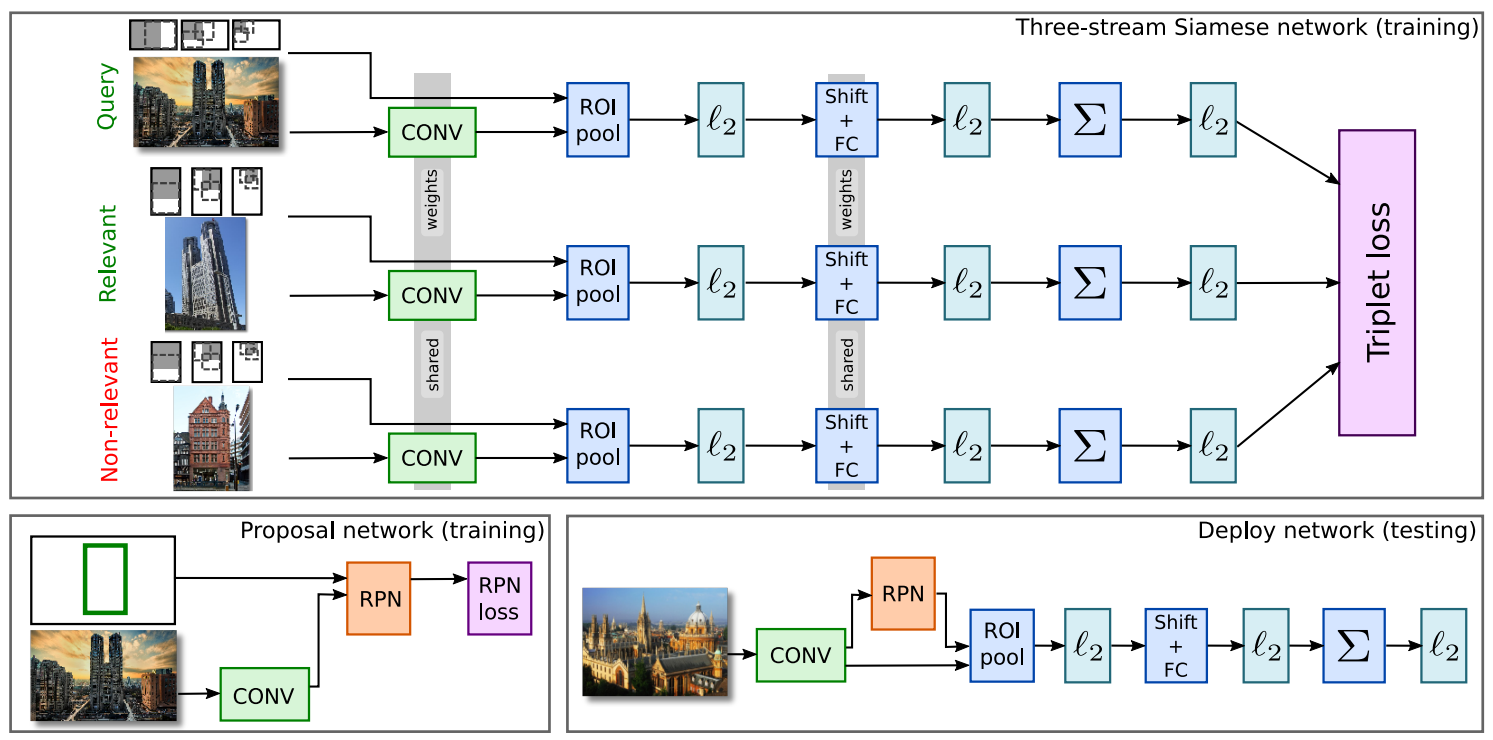
\includegraphics[width=\textwidth]{pics/Chapter2/rmac.png}
    \caption{Minh họa kiến trúc mô hình R-MAC \cite{tolias2015particular}}
\end{figure}

Cơ chế attention và lớp trọng số là một chiến lược mới, với mục tiêu chọn ra những thông tin, đặc trưng mang tính tương quan cao từ các hình ảnh để tăng hiệu năng hoạt động của các mô hình truy xuất địa danh. Khác với cơ chế chọn vùng, cơ chế attention không truy xuất thông tin từ những vùng mà mô hình cho là quan trọng, mà truy xuất tất cả các vùng trong ảnh cùng một lúc. Sau đó, các đặc trưng trích xuất được được tổng hợp lại dựa theo một lớp trọng số và điều kiện đánh giá cụ thể. Điều kiện đánh giá này, vào những ngày đầu, được thiết kế dựa theo các cơ chế phỏng đoán (heuristic) như khoảng cách so với trọng tâm hình ảnh, độ nổi bật của đặc trưng trong tất cả các kênh (channel), \dots Hướng tiếp cận này đạt nhiều thành công trong các tập dữ liệu chứa các đối tượng lặp đi lặp lại và thiếu tính tương phản cao. Ngoài ra, sự đa dạng trong phương thức thiết kế lớp trọng số cho phép nhà nghiên cứu tùy chỉnh mô hình để giải quyết các vấn đề cụ thể. Tuy nhiên, các mô hình này dễ trở nên thiếu linh hoạt, khó huấn luyện để tổng quát hóa và chỉ đạt kết quả tốt nhất khi được huấn luyện đầu-cuối (end-to-end). Ngày nay, hướng tiếp cận này thường được hiện thực sử dụng cơ chế Transformers (một loại mô hình auto-encoder), Vision Transformers (ViT)\cite{dosovitskiy2020image}, \cite{shavit2023coarse}. Nhận thấy tác động tài nguyên của ViT, \cite{alibey2023mixvpr} đề xuất sử dụng mạng học sâu MLP-Mixer \cite{tolstikhin2021mlpmixer}, một mạng học sâu sử dụng nhiều lớp MLP (Multi-Layer Perceptron) kết nối đầy đủ (fully-connected) với nhau, để thay thế cho ViT với mục tiêu đạt được cùng hiệu năng nhưng đòi hỏi ít tài nguyên hơn. Tác giá của \cite{alibey2023mixvpr} cho rằng với tác vụ truy xuất địa danh, MLP-Mixer là một lựa chọn có tiềm năng cao để thay thế cho ViT.

\begin{figure}[H]
    \centering
    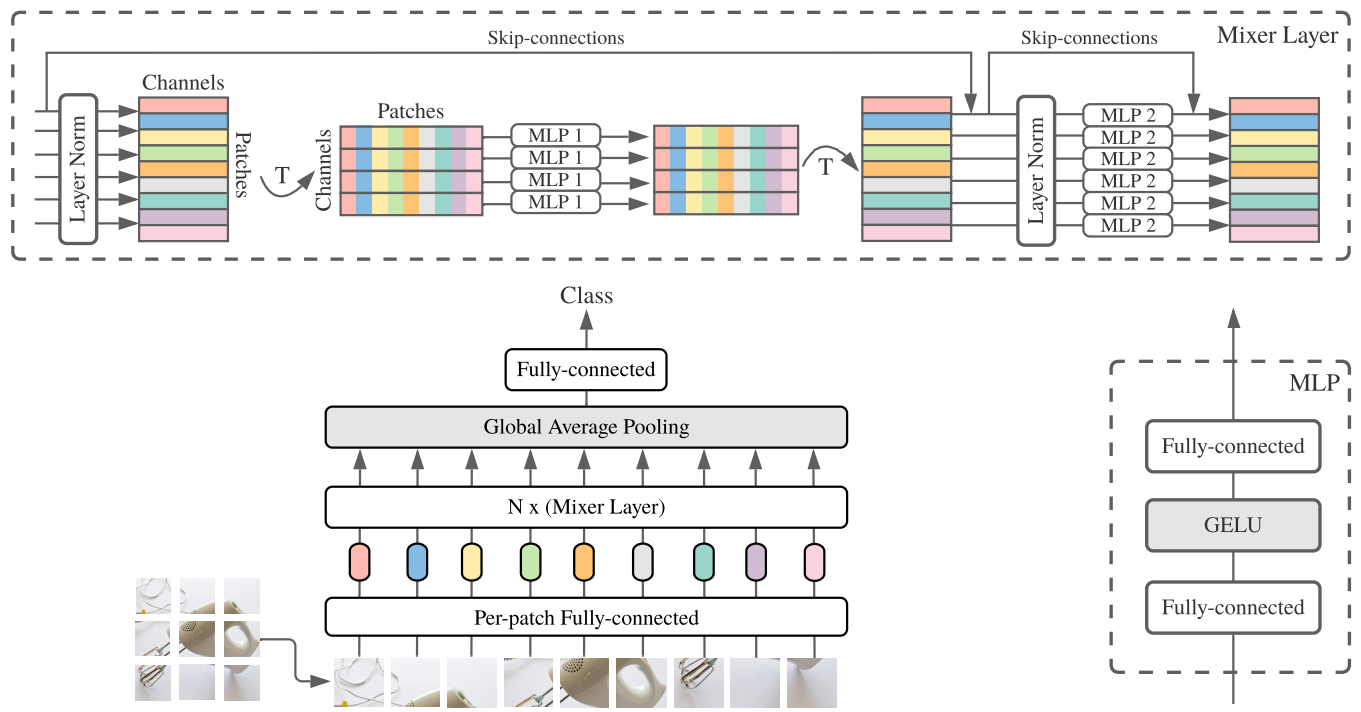
\includegraphics[width=\textwidth]{pics/Chapter2/mlpmixer.png}
    \caption{Minh họa kiến trúc mô hình MLP-Mixer \cite{tolstikhin2021mlpmixer}}
\end{figure}

\subsubsection{Góc nhìn ảo và sự biến dạng}

Trong thực tế, các đặc trưng cục bộ dày đặc được sử dụng cho quá trình so sánh tương quan, mặc dù mạnh hơn so với các đặc trưng cục bộ thưa thớt trước các thay đổi về ánh sáng \cite{zhou2016evaluating}, song không thu hẹp được các ảnh hướng đến từ biến đổi hình học (tỷ lệ và góc nhìn). Đối mặt với vấn đề này, một số bài báo \cite{torii201524, taira2018inloc} đề xuất các chiến thuật sinh góc nhìn (view synthesis). Dựa vào cơ sở dữ liệu chứa ảnh RGB và thông tin độ sâu, các mô hình này truy xuất một danh sách các ví trí sơ bộ gần đúng và chế tạo góc nhìn ảo tương ứng, đưa ảnh truy vấn và ảnh truy xuất về cùng một góc nhìn. Quá trình lựa chọn ảnh khớp tốt nhất được thực hiện một cách đơn giản, trực tiếp lên số lượng các điểm ảnh trùng và không trùng của các ảnh. Mặc dù hướng tiếp cận này tạo ra số lượng lớn các dị vật trong ảnh (visual artifacts), chiến thuật này thường đạt kết quả tốt hơn so với các mô hình truy xuất địa danh cơ bản.

Ngoài ra, trong các ứng dụng đặc biệt hơn như truy xuất vị trí từ các góc nhìn chéo, các mô hình cần phải truy vấn ảnh lấy được từ các góc nhìn trên không để so sánh với ảnh lấy được từ góc nhìn trên mặt đất và ngược lại. Sự khác nhau rất lớn về góc nhìn này đã tạo nên không ít khó khăn. Một giải pháp cho vấn đề này là quá trình chiếu tất cả các ảnh về một góc nhìn chung \cite{lin2015learning, castaldo2015semantic}. Một giải pháp khác sử dụng thêm các đặc trưng chỉ hướng (rolling descriptor) cho quá trình truy vấn để mã hóa thông tin chỉ hướng vào đặc trưng biểu diễn của các ảnh trong cơ sở dữ liệu \cite{xia2023convolutional}. Trong quá trình suy luận (inference), mô hình này khai phá thông tin chỉ hướng từ các ảnh góc rộng (panorama) để mã hóa vào biểu diễn truy vấn, so sánh tương quan giữa các đặc trưng biểu diễn này với các đặc trưng biểu diễn của các ảnh trong cơ sở dữ liệu.

\subsubsection{Thông tin ngữ nghĩa}

Việc thu thập và sử dụng thông tin ngữ nghĩa được đánh giá rất cao trong các hướng tiếp cận của bài toán. Thông tin này hỗ trợ trực tiếp quá trình chọn vùng và các điểm ảnh quan trọng như một yếu tố heuristic, cho phép các mô hình phát triển độ bền vững của mình trước các tác động môi trường và thay đổi trong điều kiện khách quan. Các hướng tiếp cận hiện đại ngay nay thường sử dụng triệt để mọi thông tin mà môi trường truy xuất cung cấp như thông tin về độ sâu, thông tin về mùa màng, thời gian, ánh sáng, \dots Ngoài ra, các loại thông tin như độ liên quan giữa số lượng, sự hiện diện của các phương tiện giao thông, các kiến trúc lặp đi lặp lại cũng hỗ trợ đáng kể cho quá trình lọc đặc trưng, loại bỏ các yếu tố gây nhiễu, lựa chọn các cột mốc địa danh có tính tương quan cao.

\subsubsection{Thông tin về độ sâu}

Thông tin độ sâu thường được xem là dữ liệu đi kèm với các tập dữ liệu truy xuất địa danh. Đóng vai trò là cầu nối giữa hình ảnh hai chiều và thông tin ba chiều của địa danh, thông tin độ sâu thường được sử dụng để tăng độ bền cho các mô hình học sâu trước các thay đổi về điều kiện ảnh. Ngoài ra, độ sâu còn có thể được tích hợp vào các đặc trưng biểu diễn để hỗ trợ quá trình trích xuất biểu diễn toàn cục cho quá trình truy xuất hình ảnh. Tuy nhiên, giống với các mô hình học từ dữ liệu thu thập được từ cảm biến độ sâu như LiDAR, việc đòi hỏi dữ liệu huấn luyện chứa thông tin về độ sâu là một hạn chế lớn, giảm khả năng mở rộng cho tập dữ liệu vì các vấn đề thu thập, lưu trữ, cập nhật và huấn luyện. Vì lý do này, một số hướng tiếp cận trong bài toán thường thiết kế các mô đun học sâu phụ cho mô hình của mình, với mục đích tự xây dựng lại một phiên bản cơ bản hơn của thông tin này trong quá trình huấn luyện. Sử dụng phương pháp tiếp cận này, mô hình chỉ cần nhận vào ảnh 2 chiều RGB trong quá trình truy xuất\cite{piasco2019learning}.

\subsubsection{Thích nghi với điều kiện môi trường thay đổi}

Những thách thức mà các mô hình truy xuất địa danh phải đối mặt khi đối mặt với các thay đổi về điều kiện môi trường như ánh sáng, thời tiết và mùa màng được công nhận rộng rãi \cite{zaffar2019levelling} và vẫn còn đươc xem là một vấn đề mở. Một lượng lớn các tài liệu đã nghiên cứu các hạn chế của các đặc trưng học sâu trong các điều kiện khó khăn \cite{zhou2016evaluating, sunderhauf2015performance, chen2017deep} và các phân tích này đã cung cấp một số hướng dẫn để tìm ra các đặc trưng mạnh mẽ hơn. Các nhà nghiên cứu cho rằng, các đặc trưng cục bộ cần phải được phân bố một cách dày đặc mới có thể tránh khỏi vấn đề hiệu năng kém trước các thay đổi về độ sáng (ngày/đêm). Đồng thời, một giải pháp thay thế hiệu quả là quá trình tiền xử lý dữ liệu ảnh đầu vào bằng một mô hình học sâu đơn giản, với mục tiêu chuẩn hóa độ sáng của ảnh. Một số đánh giá xếp hạng cho thấy, các đặc trưng học sâu có hiệu năng tốt hơn trước khi được so sánh với các đặc trưng được thiết kế thủ công \cite{arandjelovic2017netvlad}. \cite{taira2018inloc} ghi nhận rằng đặc trưng cục bộ dày đặc hoạt động tốt trong môi trường trong nhà, nơi thiếu các đặc trưng lặp đi lặp lại và đặc trưng bề mặt vật liệu (texture) trong khi các mô đun trích xuất đặc trưng (feature extractions) hoạt động tốt hơn trong môi trường ngoài trời, khai thác các yếu tố ít thay đổi như kiến trúc và đặc điểm của đường phố. Một số hướng phát triển có tiềm năng sử dụng các mô hình có cơ chế tập trung lên những phần nhỏ của một ảnh như \cite{sunderhauf2015place, chen2017only, khaliq2019holistic} sử dụng chiến thuật vùng hấp dẫn (regions of interest), \cite{zhu2018attention, chen2017only, khaliq2019holistic, wang2019atloc, wang2022transvpr, alibey2023mixvpr} sử dụng cơ chế attention, \cite{garg2018lost, naseer2017semantics, seymour2019semantically}. Đồng thơi, sử dụng một chuỗi các hình ảnh liên tục thay cho một hình ảnh đơn lẻ cũng có tác động lớn đối với độ bền của mô hình trước điều kiện mô hình thay đổi \cite{naseer2018robust, hausler2019multi, hong2019textplace, chancan2020hybrid}.

Các giải pháp cho vấn đề thay đổi điệu kiện môi trường thường phải sử dụng các chiến thuật có yêu cầu tài nguyên lớn, khó phát triển quy mô. \cite{doan2019scalable} đề xuất một giải pháp ba bước để khắc phục các vấn đề này: xây dựng mô hình chứa cơ sở dữ liệu có thể tiếp tục mở rộng phạm vi với nhiều ảnh được thu thập ở các điều kiện môi trường khác nhau. Doan và nnk đề xuất mô hình:

\begin{enumerate}
    \item Một thuật toán nhận diện địa điểm trực quan được xây dựng dựa trên mô hình Markov ẩn (Hidden Markov Model) với hiệu năng huấn luyện và kiểm thử cao.
    \item Một chiến thuật chọn lọc điều chỉnh số lượng ảnh được thêm vào cơ sở dữ liệu, đảm bảo chỉ thêm các ảnh biểu diễn các ảnh với dữ liệu mới và chứa nhiều đặc điểm quan trọng.
    \item Một thuật toán nén hợp nhất các phần kết nối được với nhau trong cơ sở dữ liệu, giảm kích thước lưu trữ.
\end{enumerate}

\begin{figure}[H]
    \centering
    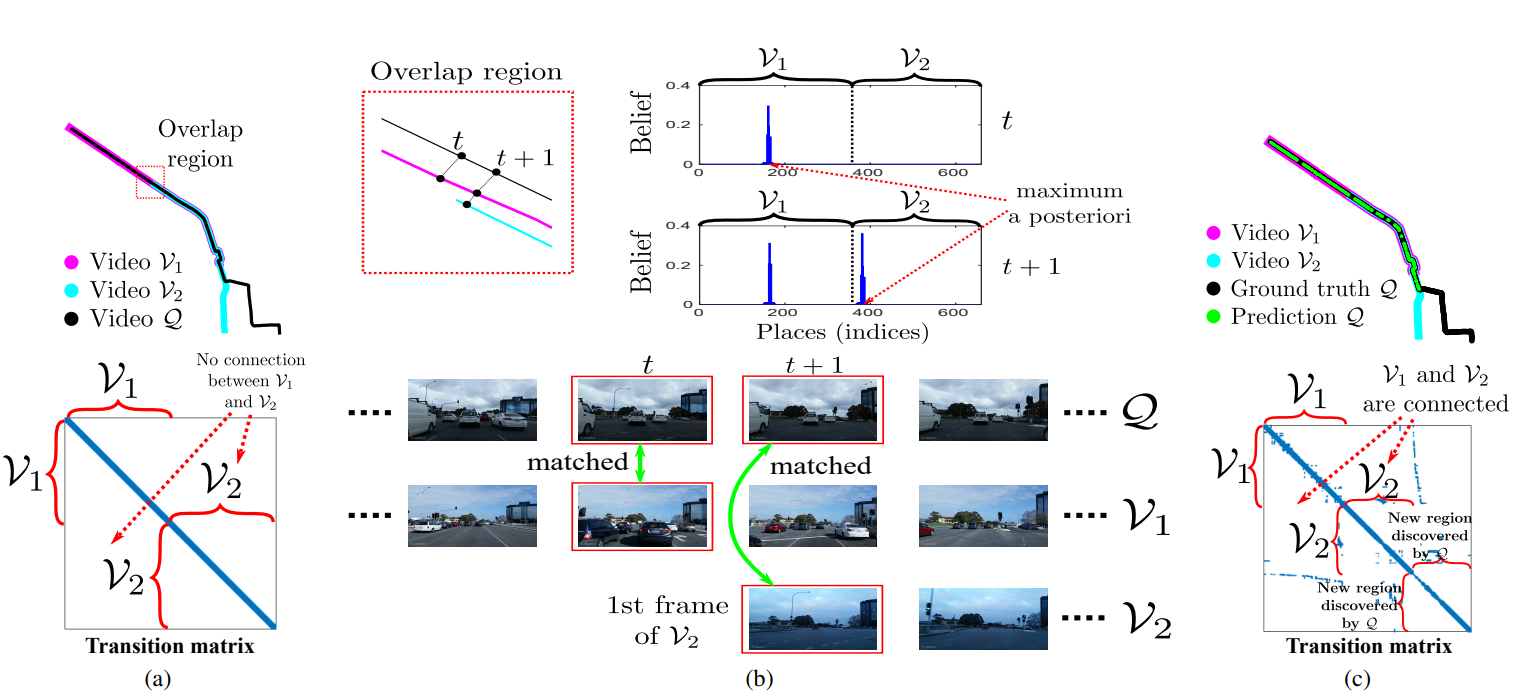
\includegraphics[width=\textwidth]{pics/Chapter2/model3step.png}
    \caption{Minh họa kiến trúc mô hình \cite{doan2019scalable}}
\end{figure}

Gần đây hơn, một số nghiên cứu tìm cách đối mặt với vấn đề này dưới góc nhìn khác, giải quyết vấn đề miền chéo, khi ảnh truy vấn chứa nhiều sự khác biệt về độ sáng, thời tiết, mùa màng hoặc thiết bị thu thập ảnh so với ảnh trong cơ sở dữ liệu. Hướng tiếp cận này đặt ra mục tiêu sinh ra ảnh mới để thay thế ảnh truy vấn, cùng mô tả một cảnh nhưng với với miền của ảnh trong cơ sở dữ liệu. Trong \cite{Porav2018AdversarialTF, Annosheh2019Night} quá trình sinh ảnh thường được thực hiện bởi mạng đối nghịch tạo sinh (GAN). Thay vì căn chỉnh dữ liệu các miền khác nhau, một hướng tiếp cận khác đặt trọng tâm trong quá trình học đặc trưng đa miền và tách cụm những đặc trưng phụ thuộc vào điều kiện môi trường và những đặc trưng bất biến \cite{yin2019multi}. Mạng đối nghịch tạo sinh đạt hiệu quả đáng kể đối với các vấn đề miền chéo chứa sự khác biệt về độ sáng, thời tiết hoặc mùa màng nhưng chưa giải quyết được vấn đề miền chéo chứa sự khác biệt về thiết bị thu thập. Trong thực tế, các tập dữ liệu huấn luyện mô hình luôn được thu thập trong khoảng thời gian sớm hơn so với dữ liệu truy vấn. \cite{wang2019attention} đề xuất kiến trúc sử dụng một mô hình trích xuất đặc trưng học sâu tích chập với lớp aggregation VLAD \cite{jegou2010aggregating} và hai mô đun chủ chốt:

\begin{itemize}
    \item một mô đun attention đánh giá độ quan trọng của các đặc trưng tổng hợp được từ lớp VLAD, và
    \item một hàm mất mát thích nghi miền sử dụng hàm khác biệt trung bình tối đa đa hạt nhân (multi-kernel maximum mean discrepancy hoặc MK-MMD) hỗ trợ mạng học được không gian chung của cả hai miền.
\end{itemize}

Trong đó, mô đun attention được đánh giá có cống hiến ít so với cải tiến chung của mô hình trong khi hàm mất mát nắm vị trí trọng tâm.

\begin{figure}[H]
    \centering
    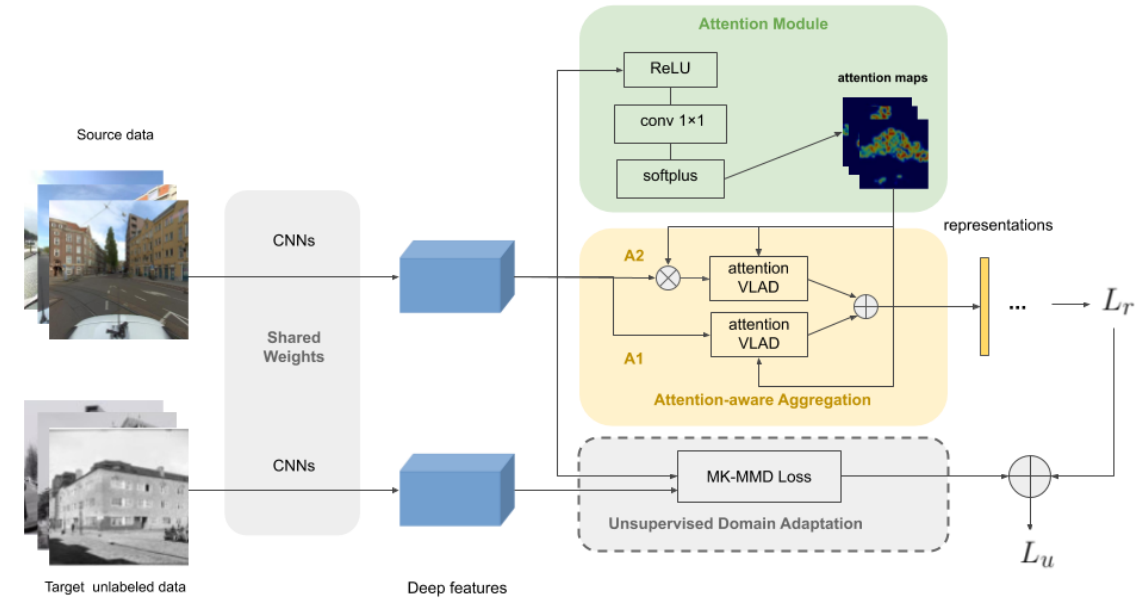
\includegraphics[width=\textwidth]{pics/Chapter2/cnn160.png}
    \caption{Minh họa kiến trúc mô hình \cite{wang2019attention}}
\end{figure}

Thêm vào đó, đặt vấn đề dưới góc nhìn của quá trình thu thập dữ liệu, \cite{hu2020dasgil} đề xuất sử dụng tập dữ liệu ảo chứa thông tin độ sâu và thông tin ngữ nghĩa để huấn luyện mô hình học sâu. Quá trình huấn luyện lấy cảm hứng từ mô hình đối nghịch đảm bảo đặc trưng trích xuất được từ miền ảo và miền ảnh thật có độ phân bố tương tự nhau.

Trong \cite{PAOLICELLI-2022-FRONTIERS}, Berton và nnk chứng minh hướng tiếp cận áp dụng kết hợp cả bài toán sinh dữ liệu (generative) và bài toán thích ứng miền (domain adaptation) có khả năng tăng hiệu năng của các mô hình cao.
